\section{Framework}
\label{sec:model}

Fig.~\ref{fig:arch} summarises the framework. A sensor node at a remote river site records several water-quality parameters. At the end of each day it selects the fewest readings from which the server can reconstruct every reading within a tolerance, packs them into messages, and adds redundancy. The satellite link delivers each message or loses it, and the node never learns which. The server decodes what arrived, reconstructs the record, and states which readings it can certify; agencies then take decisions that use only certified readings.

\begin{figure}[t]
\centering
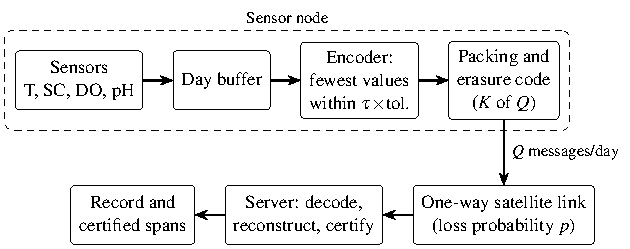
\includegraphics[width=\textwidth]{figs/arch.pdf}
\caption{Workflow of the framework. The node never learns which messages arrived; the server uses only the bytes that arrived and the site profile (the sampling interval of each parameter).}
\label{fig:arch}
\end{figure}

\subsection{Record, tolerance, and reconstruction}
\label{sec:record}
A channel-day is one parameter $j$ of one site on one UTC day, with readings $x_j(t)$, $t = 0, \dots, n_j - 1$, on the parameter's own sampling grid. Each reading has a tolerance $\delta_j(t) > 0$. This study used the accuracy that the USGS requires of an excellent continuous record \citep{wagner2006}: 0.2\,\textdegree C for temperature, 3\% of the value for specific conductance, the greater of 0.3\,mg/L and 5\% of the value for dissolved oxygen, and 0.2 units for pH. The tolerance is relative to the sensor record; the accuracy of the sensor itself (calibration, fouling, and drift) is outside it.

The node quantises a kept reading to a 13-bit code (Section~\ref{sec:frame}), and the server holds the dequantised value $\tilde{x}_j(s)$. From the kept slots that reached it, $s_1 < \dots < s_k$, the server reconstructs $\hat{x}_j(t)$ by holding $\tilde{x}_j(s_1)$ back to midnight, interpolating linearly between consecutive kept slots, and holding $\tilde{x}_j(s_k)$ to the end of the day. Each day is therefore self-contained: no value of the previous day is needed. Chaining days, in which each day starts from the previous day's last value, saved \chainSaveDev{} values per day on \chainPairsDev{} pairs of consecutive development days. However, at six messages per day and a loss probability of 0.3, a chained day was fully certified \chainGainLoDev{} to \chainGainHiDev{} less often, because its first span depends on the previous day's final message; bursts across midnight affected it most. The normalised error of a reading is
\begin{equation}
e_j(t) = \frac{|x_j(t) - \hat{x}_j(t)|}{\delta_j(t)}.
\label{eq:err}
\end{equation}

\subsection{Encoder}
\label{sec:encoder}
For a level $\tau$, the encoder selects for each parameter the fewest slots $S_j(\tau)$ whose reconstruction keeps $e_j(t) \le \tau$ for every reading; the record of a day is the union of these sets at $\tau = 1$, listed in a fixed planned order (temperature, dissolved oxygen, pH, specific conductance; then time). Three features make the bound exact and the record self-contained:
\begin{itemize}
  \item Quantisation: every candidate error is computed with the dequantised endpoint values that the server will hold; therefore, the bound includes quantisation and needs no margin.
  \item Head and tail: the first kept value is held back to midnight and the last is held to the end of the day; thus, a flat parameter costs one value and no anchor from the previous day is used.
  \item Censoring: a reading outside the quantiser range (for example a sensor fault reported as a negative concentration) is always kept, carried as its flag code, excluded from the bound, and reported by the server as below or above range.
\end{itemize}
The selection is the minimum-number problem of polygonal approximation \citep{imai1988}, here with per-reading tolerances. It was solved exactly by a forward dynamic program: for a fixed start, a span to a later slot keeps every reading in between within tolerance exactly when the slope of the span lies in the intersection of the slope windows imposed by those readings \citep{orourke1981}, an intersection that only shrinks as the span grows. Head and tail spans are checked with prefix and suffix intervals. The encoder needs $O(n^2)$ time and $O(n)$ memory per channel-day; it reproduced the plans of a reference implementation built on a full error table on all \nDaysDevAll{} record days of the development year.

\subsection{Message frame}
\label{sec:frame}
Each message carries the 23-byte user payload of the KIM1 module \citep{kineis2023kim1}. The operator delivers it with the device identifier and the time of reception at the satellite \citep{kineis2024formats}; neither is in the payload. Table~\ref{tab:frame} provides the layout. A three-byte header identifies the day block, the message, and the number of data units $K$. The remaining 20 bytes form a unit that is protected as a whole by the erasure code. A unit carries a CRC-16 computed over its content and its context (block day, $K$, and unit index), such that a unit recovered from a corrupted or misassociated message is rejected. It then carries up to three segments, each holding consecutive values of one record day with the position of its first value in the planned order. Values carry their parameter, slot, and reading. Linear grids are decimal (0.01\,\textdegree C, 0.005\,mg/L, and 0.002 pH units); thus, readings reported at 0.1 or 0.01 are carried exactly. Specific conductance uses a logarithmic grid whose step is 0.14\% of the value. The worst quantisation error is 2.5\% of the tolerance. A unit holds five values (three in a 19-byte payload); the header and integrity fields take 35\% of the payload.

\begin{table}[t]
\centering
\caption{Message frame (23-byte payload).}
\label{tab:frame}
\small
\begin{tabularx}{\textwidth}{@{}llX@{}}
\toprule
Part & Bits & Fields \\
\midrule
Header (not coded) & 24 & version (2); block day modulo 64 (6); message index (7); $K$ (7); coded (1); code type (1) \\
Unit check & 16 & CRC-16 over the unit and its context \\
Segment count & 2 & 0 to 3 segments \\
Segment header & 21 & day offset from the block day (6); first planned position (10); value count (3); last value of the day (1); record within tolerance (1) \\
Value & 24 & parameter (2); slot (9); reading code (13; codes 0 and 8191 flag a reading below or above range) \\
Padding & & zeros to 20 bytes \\
\bottomrule
\end{tabularx}
\end{table}

The block day is unwrapped from the operator's reception time, which is unambiguous while the delay from sending to reception is below 63 days and the node clock is within one day of UTC. The planned positions let the server know exactly which values it lacks without any feedback.

\subsection{Delivery designs}
\label{sec:designs}
A plan allows $Q$ messages per day. Let $D_1$ be the number of units that the day's record occupies. The proposed design, the record-first code, sends the $D_1$ data units and $Q - D_1$ parity messages of a systematic Reed--Solomon code over GF($2^8$) \citep{reed1960}; any $D_1$ of the $Q$ messages recover the record. $D_1$ changes from day to day and travels in every header. Days whose record exceeds $Q$ units send their first $Q$ units, which yield partial certificates only. Table~\ref{tab:designs} lists the baselines, which use the same frame and quota.

\begin{table}[t]
\centering
\caption{Delivery designs compared (same frame and the same $Q$ messages per day).}
\label{tab:designs}
\small
\begin{tabularx}{\textwidth}{@{}lX@{}}
\toprule
Design & Content and transmission \\
\midrule
Record-first code (proposed) & The record; $D_1$ data units and $Q - D_1$ Reed--Solomon parity messages. \\
Record-first fountain code & The record; $D_1$ data units and $Q - D_1$ random linear combinations over GF($2^8$) \citep{luby2002,ho2006}. \\
Record-first repetition & The record; units sent round robin over all $Q$ messages (copies interleaved); also in block order. \\
Fixed-$K$ code & The fewest values at the smallest level $\tau$ that fills $5K$ values; $K$ data units and $Q - K$ parity; $K$ chosen without knowledge of the channel. \\
Fixed-$r$ repetition & As the fixed-$K$ code for $\lfloor Q / r \rfloor$ units, repeated round robin. \\
Reliable-link design & The fewest values at the smallest $\tau$ that fills $5Q$ values, each unit sent once: optimal when no message is lost \citep{deligiannakis2007}. \\
Tag practice & A fixed number of broken-stick points per parameter (endpoints first, then the largest absolute deviation), with units picked pseudo-randomly with replacement for each transmission, as satellite-linked animal tags do \citep{boehme2009,photopoulou2015}; a seven-day buffer version rotates units over the following week. \\
Every $k$-th reading & Every $k$-th reading of every parameter, newest included, $k$ as small as the quota allows. \\
\bottomrule
\end{tabularx}
\end{table}

\subsection{Decoding and certification}
\label{sec:cert}
The server keeps the majority header of each block, accepts only units that pass their CRC, and decodes the erasure code when sufficient messages arrived, retrying other parity messages if a recovered unit fails its check. It then certifies readings from the received planned positions alone:
\begin{itemize}
  \item a span between two consecutive planned positions of the same parameter is certified when both arrived;
  \item the head of a parameter is certified when its first planned value arrived and is known to be first (position 0, or the preceding position arrived and belongs to another parameter);
  \item the tail is certified when its last planned value arrived and is known to be last (the next position belongs to another parameter, or the segment carries the last-value flag);
  \item censored readings are reported as below or above range and never certified.
\end{itemize}

Proposition 1 (soundness): if the record keeps every reading within tolerance, every value used arrived as transmitted, the block day was unwrapped correctly, the site profile is correct, and each day has one record, then every certified reading satisfies $e_j(t) \le 1$ in Eq.~(\ref{eq:err}). The reconstruction on a certified span depends only on the two received values that bound it, which are the values the encoder used; therefore, the encoder's bound carries over. A day is fully certified exactly when all its planned values arrived.

Proposition 2 (record-first coding needs no knowledge of the channel): among designs whose messages carry linear combinations of the record's $D_1$ units, no design fully certifies a day with probability greater than $P(N \ge D_1)$, where $N$ is the number of messages that arrive, and the record-first code attains this bound for every loss process, including bursty and correlated loss. Recovering $D_1$ unknown units requires at least $D_1$ received combinations, and a maximum-distance-separable code recovers them from any $D_1$ messages.

The study distinguished four quantities, which are easy to conflate:
\begin{itemize}
  \item the record error, $\max e_j(t)$ over the record, which the encoder knows exactly;
  \item full certification, which the server establishes from the received bytes;
  \item the share of days within tolerance as judged by an observer who knows the full sensor record, which includes days that are within tolerance by chance but cannot be verified;
  \item the probability of full certification under a stated loss model, $G_{\mathrm{cert}}$, which is the primary outcome.
\end{itemize}
No design guarantees delivery over a one-way link that loses messages; Proposition 1 guarantees that whatever the server certifies is within tolerance.

\subsection{Decisions from certified records}
\label{sec:decisions}
A certified reading bounds the true reading: because $|x - \hat{x}| \le \delta(x)$ with $\delta(x) = \max(a, r|x|)$ for the constants $a$ and $r$ of each parameter, the server can compute an interval that contains $x$ from $\hat{x}$ alone. For a criterion such as a daily minimum of dissolved oxygen below 5\,mg/L, the server therefore states one of three outcomes: certainly exceeded (some certified interval lies entirely below the threshold), certainly not exceeded (every reading is certified and every interval lies above it), or undetermined. The first two cannot be wrong under the conditions of Proposition 1. Designs without a bound can only compare their reconstruction with the threshold.
